\section{Einführung}

	\subsection{Entstehung von Myonen}
	\textit{Myonen} $\mu{\pm}$ lassen sich im heute gängigen Standardmodell der Teilchenphysik zur zweiten Generation der elektrisch geladenen Leptonen zuordnen. Sie sind mit $m_\mu = 105,658\ \unit{MeV = 206,768\ m_e}$\cite{pdg} die schweren Pendants zum Elektron.\\
	Im folgenden Versuch werden Myonen aus der kosmischen Höhenstrahlung, welche zu 85\% aus hochenergetischen Protonen besteht, untersucht. Bei Zusammenstößen dieser Protonen mit Atomkernen in der Erdatmosphäre entstehen die geladenen $\pi^\pm$-Mesonen Reaktionen niedrigster Ordnung sind:
		\begin{align*}
			&p + p \longrightarrow p + n + \pi^+\\
			&p + n \longrightarrow p + p + \pi-
		\end{align*}
	Diese Mesonen zerfallen nach etwa $2,6\cdot10^{-8}\ \unit{s}$ über die schwache Wechselwirkung. Der mit einem Anteil von 99,988\% dominierende Zerfallskanal endet in einem Myon und einem zugehörigen Neutrino und kann mit folgender Zerfallsgleichung und dem Feynmandiagramm in Abbildung \ref{fig:pionzerfall} beschrieben werden:
		\begin{align*}
			&\pi^+ \longrightarrow \mu^+ + \nu_\mu\\
			&\pi^- \longrightarrow \mu^- + \bar{\nu}_\mu\\
		\end{align*}
		\begin{figure}[hp]
					\centering
					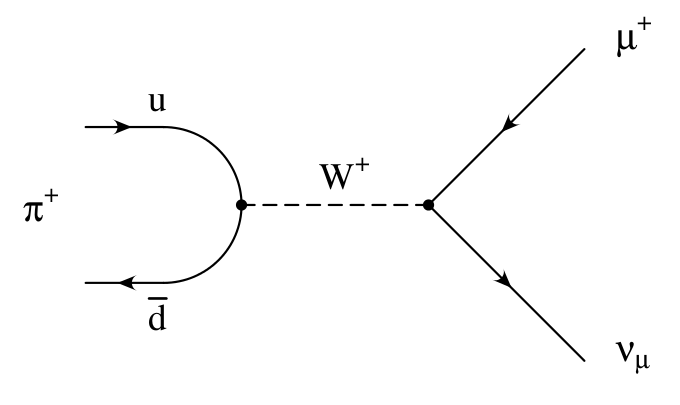
\includegraphics[width = 0.7\linewidth]{pic/pionzerfall.png}
					\caption{Feynman-Diagramm des Antimyonenzerfalls.}
					\label{fig:pionzerfall}
		\end{figure}
		
	\subsection{Zerfall von Myonen}
	Da das Myon ein sehr schweres Teilchen ist, zerfällt es nach einer sehr kurzen Zeit von:\cite{PA}\\
		\begin{equation} \label{eq:lit}
			\tau_\mu = (2,19703 \pm 0,00004)\ \unit{\mu s}
		\end{equation}
	mit nahezu 100\% über den schwachen Zerfall, der mit Hilfe der Reaktionsgleichungen (\ref{eq:mup}) und (\ref{eq:mum}) und zugehörigem Feynmangraph (nur niedrigste Ordnung) in Abbildung \ref{fig:myonzerfall} beschrieben werden kann.\\
	
		\begin{align}
			&\mu^+ \longrightarrow e^+ + \nu_e + \bar{\nu}_\mu 		\label{eq:mup}\\
			&\mu^- \longrightarrow e^- + \bar{\nu}_e + \nu_\mu 		\label{eq:mum}
		\end{align}
		\begin{figure}[hp]
			\centering
			\scalebox{0.5}[0.5]{
			\input{pic/myonzerfall.pdf_tex}
			}
			\caption{Feynman-Diagramm des Antimyonenzerfalls.}
			\label{fig:myonzerfall}
		\end{figure}
	\ \\
	Auch wenn die in Gleichung (\ref{eq:lit}) angegebene Lebensdauer sehr kurz erscheint, ist der Myonenfluss auf Meereshöhe mit $170\ \unit{Myonen/(m^2s)}$ sehr hoch. Dies lässt sich dadurch erklären, dass die oben angegebene Lebensdauer im Laborsystem der Beobachter auf der Erde angegeben ist. Da sich Myonen mit relativistischen Energien bewegen, besitzen sie in ihrem Ruhesystem eine \textit{zeitdilatierte Lebensdauer}, welche ausreicht, um an die Erdoberfläche zu gelangen. Selbst in der theoretischen Vorhersage der Lebensdauern mit Hilfe von \textit{Übergangsmatrixelementen} $\Gamma_{fi} = 1/\tau_{fi}$ (d.h. bei Übergang von Zustand $\ket{i}$ in $\ket{f}$) treten Terme auf, die nicht lorentzinvariant sind.
	
	\subsection{$\mu^-$-Einfang}
	Im Falle der negativ elektrisch geladenen Myonen $\mu^-$ existiert in Materie allerdings ein weiterer 'Zerfallskanal', der sogenannte $\mu^-$-Einfang, bei dem ein einfallendes Myon im Coulombfeld eines Atoms eingefangen wird, bis in den Grundzustand vordringt und anschließend vom Kern absorbiert wird. Dabei findet folgende Kernumwandlung(Abbildung \ref{fig:myoneinfang}) statt:
		\begin{equation*}
			\mu^- + p \longrightarrow  \nu_\mu + n 
		\end{equation*}
		
		\begin{figure}[ht]
			\centering
			\scalebox{1.}[1.]{
			\input{pic/myoneneinfang.pdf_tex}
			}
			\caption{Feynman-Diagramm des Myoneneinfangs.}
			\label{fig:myoneinfang}	
		\end{figure}
	\ \\
	Ist $\Gamma_z = 1/\tau_z$ die Partialbreite  des schwachen Zerfallskanals (\ref{eq:mum}) und $\Gamma_e=1/\tau_e$ die des $\mu^-$-Einfangs, ergibt sich die totale Breite des $\mu^-$-Zerfalls zu:
		\begin{align}
			&\Gamma_{\mu^-} = \Gamma_z + \Gamma_e\\
			&\tau_{\mu^-} = \left(\frac{1}{\tau_z} + \frac{1}{\tau_e}\right)^{-1} < \tau_{\mu^+}  
		\end{align}
	Im Praktikumsversuch werden die Myonen mit einer Kupferplatte eingefangen. Da der $\mu^-$-Einfang dafür sorgt, dass nach etwa $1\ \unit{\mu s}$ alle negativ geladenen Fermionen eingefangen worden, dominieren die $\mu^+$-Zerfälle die Messung. 
	
	\subsection{Messprinzip und Versuchsaufbau}
	%TODO@Christian: Kurz beschreiben wie Szintillator und PM funktioniert + Versuchsaufbau (nur Messaufbau 1)